%%%% Proceedings format for most of ACM conferences (with the exceptions listed below) and all ICPS volumes.
\documentclass[sigconf]{acmart}
\usepackage{graphicx, wrapfig, floatflt}
\graphicspath{{imgs/}}
\usepackage[para]{footmisc} %  footnotes na mesma linha
\usepackage{stfloats}
\usepackage{enumerate}

\usepackage[most]{tcolorbox}
\usepackage[english,ngerman,brazilian]{babel}


\newtcolorbox[blend into=figures]{card}[2][]{enhanced,
  float=tbp,title={#2},
  colframe=gray!75!black,olback=yellow!5!white,#1
}


\settopmatter{printacmref=false}
\setcopyright{none}
\renewcommand\footnotetextcopyrightpermission[1]{}
\pagestyle{plain}
\captionsetup{justification   = raggedright,
              singlelinecheck = false}
\newcommand{\source}[2]{\raggedleft{}\vspace*{-7mm}\caption*{ \textmd{\scriptsize{Dados: {#1}.\hfill Ferramenta:{#2}}}}}
\def\BibTeX{{\rm B\kern-.05em{\sc i\kern-.025em b}\kern-.08emT\kern-.1667em\lower.7ex\hbox{E}\kern-.125emX}}

% end of the preamble, start of the body of the document source.
\begin{document}

%
% The "title" command has an optional parameter, allowing the author to define a "short title" to be used in page headers.
\title[Fronteiras da Transferência de Aprendizado: uma revisão sistemática com enfoque meta-analítico]{Fronteiras da Transferência de Aprendizado: \\
uma revisão sistemática com enfoque meta-analítico}
%

\author{Fred Guth}
\email{fredguth@fredguth.com}
\affiliation{%
  \institution{Departamento de Ciência de Computação, Universidade de Brasília}
  \postcode{70.910-900}
  \city{Brasília}
  \state{DF}
  \country{Brazil}
}

\renewcommand{\shortauthors}{Guth, F.}

\begin{abstract}
  Humanos e animais conseguem aprender com poucas amostras e apresentam extraordinária capacidade de generalização que os algoritmos de aprendizagem de máquina ainda estão longe de alcançar~\cite{goodfellow}. Os modelos mais bem sucedidos da atualidade exigem uma enormidade de dados bem rotulados que são caros e difíceis de obter, tornando-se hoje um dos maiores empecilhos para aplicações práticas. Tais fatos apontam para o grande potencial da área de Transferência de Aprendizado, que tem por objetivo aproveitar o conhecimento obtido em uma atividade para aprender mais eficientemente outras, que guardem alguma relação com a primeira. O presente estudo visa apresentar uma revisão sistemática da literatura e identificar, com embasamento quantitativo, as principais contribuições para a área. Além disso, usamos medidas de acoplamento bibliográfico para identificar trabalhos na fronteira do conhecimento e fizemos uma análise textual, em resumos e palavras-chave, comparando estes com os "clássicos" ~da área de forma a mapear para que direção a pesquisa avança.  
\end{abstract}


\begin{CCSXML}
<ccs2012>
 <concept>
 <concept_id>10010147.10010257.10010258.10010262.10010277</concept_id>
 <concept_desc>Computing methodologies~Transfer learning</concept_desc>
 <concept_significance>500</concept_significance>
 </concept>
</ccs2012>
\end{CCSXML}
\ccsdesc[500]{Computing methodologies~Transfer learning}

\keywords{transferência de aprendizado, revisão sistemática, enfoque meta-analítico}


\maketitle


\section{Introdução} 
  Recentes avanços em aprendizagem de máquina tornam possíveis aplicações que são capazes de reconhecer pessoas, lugares e objetos com acurácia super-humana\cite{fei}, diagnosticar câncer de pele tão bem quanto dermatologistas\cite{skin_cancer},  ver através de paredes usando sinais de rádio\cite{wifi}, entre tantas outras. Apesar de tanto sucesso, os modelos mais bem sucedidos da atualidade exigem uma enormidade de dados bem rotulados que são caros e difíceis de obter, pois, em geral, o jeito padrão de se treinar modelos é sempre começar \emph{tabula rasa}, ou seja, com uma inicialização aleatória dos parâmetros~\cite{Ruder2019Neural}. 
  
  Aprender assim, a partir do nada, é contrário à forma como os humanos o fazem. Em nosso dia a dia, transferimos conhecimento a todo momento. Saber tocar piano facilita aprender tocar órgão. Saber português ajuda a aprender espanhol. Pessoas conseguem inteligentemente aplicar conhecimento prévio para resolver novos problemas com maior eficácia e eficiência\cite{PanYang}. Algoritmos de aprendizagem de máquina ainda estão longe de alcançar essa extraordinária capacidade de generalização\cite{goodfellow}. Estudos recentes~\cite{DBLP:journals/corr/JiaL17} mostram que os algoritmos atuais não generalizam bem além de dados vistos durante o treinamento. 
  \begin{figure}[h]
    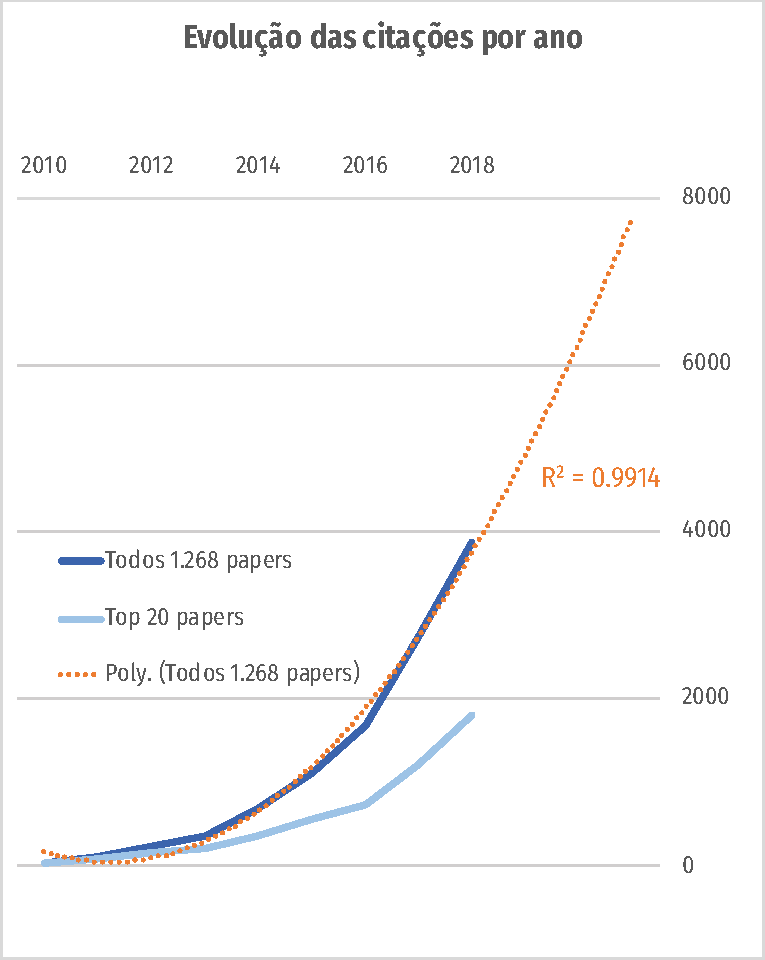
\includegraphics[width=\columnwidth]{citacoes_por_ano}
    \source{Web of Science (março/2019)}{Excel}
    \caption{Evolução do número de citações aos artigos em transferência de aprendizado nos últimos 10 anos. Até 2020, o número de citações aos artigos na área deverá dobrar.}
    \label{fig:citacoes_por_ano}
  \end{figure}

  Tais fatos apontam  o grande potencial ainda inalcançado da área de Transferência de Aprendizado (TL\footnote{Do inglês, \emph{Transfer Learning}.}), que tem por objetivo aproveitar o conhecimento obtido em uma atividade para aprender mais eficientemente outras, que guardem alguma relação com a primeira.
  
  Na prática, entretanto, TL ainda é tratada de uma forma \textit{ad hoc}, sendo os métodos de transferências meras extensões dos algoritmos de aprendizado utilizados \cite{torrey}. Essa dicotomia entre a importância do problema e a inexistência de práticas e teorias consolidadas, tornam TL um campo promissor e interessante para pesquisa. 
  
  \begin{quote} "Transferência de aprendizado será o próximo motor do sucesso comercial com aprendizado de máquinas." \hfill ---Andrew Ng, Tutorial NIPS 2016 \cite{ANg}
  \end{quote}

  Portanto, não é de se estranhar o crescente interesse pelo assunto (vide figuras \ref{fig:citacoes_por_ano} e \ref{fig:artigos_por_ano}).  

  \subsection{Objetivo}\label{objetivos}
   Esta pesquisa quer responder duas perguntas:
    \begin{enumerate}
      \item{Quais são as fronteiras do conhecimento em transferência de aprendizado?}
      \item {É possível embasar essa avaliação em dados bibliométricos?}
    \end{enumerate}
    Para responder estas perguntas é preciso, antes, analisar a literatura do tema, revelar as principais contribuições na área e como se relacionam.
  
  \subsection{Contribuições}

    \begin{enumerate}[C1.]
      \item Apresentamos uma revisão sistemática atualizada da literatura em Transferência de Aprendizagem, usando a abordagem TEMAC (\S \ref{TEMAC}). Esse método nos permite focar nas contribuições de alto impacto. 
      \item Estendemos o TEMAC com uma análise textual de resumos (\S \ref{detalha}\ref{analiseTextual}), utilizando o \emph{ScatterText}~\cite{kessler2017scattertext}, o que até onde sabemos, é uma aplicação original desta ferramenta de visualização.
      \item Apontamos com embasamento quantitativo as direções das frentes de pesquisa da área e apontamos lacunas e problemas em aberto.
    \end{enumerate}
  
  \subsection{Visão Geral e Organização do Artigo}
  Ainda nesta breve introdução apresentaremos os \emph{Trabalhos Relacionados} (\S\ref{related}). Na próxima seção (\S\ref{TEMAC}), apresentaremos o método de pesquisa que dá embasamento quantitativo que queremos para atingirmos nossos objetivos (\S\ref{objetivos}). Na seção \S\ref{literatura}, apresentamos os resultados, que são a própria  \emph{Revisão da Literatura}. \emph{Problemas em Aberto} são discutidos na seção \S\ref{emAberto}. Por fim, concluímos o trabalho (\S\ref{conclusao}) apresentando as respostas às perguntas de \S\ref{objetivos}.
  

  \subsection{Trabalhos Relacionados}\label{related}
  Pan, S. (2009)\cite{PanYang} é a mais citada revisão sobre \emph{Transferência de Aprendizado}. Hohman, F. (2018)\cite{hohman2018visual} faz uma revisão sistemática da literatura sobre análises visuais em \emph{deep learning} e utiliza um método bastante interessante baseado nos cinco W's e um H (Why, Who, What, How, When, and Where). Ruder, S. (2019) \cite{Ruder2019Neural} apresenta um capítulo com uma revisão bibliográfica e taxonomia para o contexto de NLP. Park, I. (2018)\cite{park2018identifying} utiliza uma abordagem meta-analítica para identificar a fronteira de pesquisa em \emph{Pattern Recognition}.
\section{Método: Revisão com Enfoque Meta-Analítico Consolidado}\label{TEMAC}
Na presente pequisa utilizamos o método de revisão sistemática da Teoria do Enfoque Meta-Analítico (TEMAC) ~\cite{Mariano}, que visa oferecer um embasamento quantitativo para a escolha da literatura. Apesar do nome, TEMAC não deve ser confundida com \textbf{meta-análise}, pois o foco desta é gerar conhecimento por meio de dados empíricos secundários, enquanto o daquela é oferecer uma sistematização da escolha bibliográfica.

A abordagem TEMAC é dividida em 3 etapas: 
\begin{enumerate}[a)]
  \item preparação da pesquisa;
  \item apresentação e inter-relação dos dados;
  \item detalhamento, modelo integrador e validação por evidências.
\end{enumerate}

\subsection{Preparação da Pesquisa}
Foi realizada uma busca na base de dados \emph{Clarivate Analyticis Web of Science (WoS)}, conforme especificado na figura \ref{card:wos}, no dia 31 de março de 2019, que resultou em 1.289 artigos encontrados. Nota-se que o tema é de crescente interesse (figura \ref{fig:artigos_por_ano}) e projeta-se que em 3 anos o número de artigos irá praticamente dobrar (crescimento exponencial com $R^2=0,9789$). 
\begin{figure}[htp]

\begin{tcolorbox}[colback=yellow!5!white,colframe=gray!75!black,title={Results: 1,289 (from Web of Science Core Collection)}]
  \footnotesize{
    \begin{verbatim}
    You searched for: 
    TOPIC: ("transfer learning")
    Refined by: 
    WEB OF SCIENCE CATEGORIES: 
      ( COMPUTER SCIENCE ARTIFICIAL INTELLIGENCE )
    AND LANGUAGES: ( ENGLISH ) 
    AND RESEARCH AREAS: ( COMPUTER SCIENCE )
    Timespan: 2009-2019. 
    Indexes: SCI-EXPANDED, CPCI-S, ESCI.
    \end{verbatim}
  }

\end{tcolorbox}
\caption{"Busca10anos": Parâmetros de busca na base \emph{Web of Science}.}
\label{card:wos}
\end{figure}

Também fizemos uma busca mais restrita aos trabalhos mais recentes (figura \ref{card:sota}) para a análise das \emph{Fronteiras de Pesquisa} (\S\ref{fronteiras}).
\begin{figure}[htp]
  \begin{tcolorbox}[colback=yellow!5!white,colframe=gray!75!black,title={Results: 384 (from Web of Science Core Collection)}]
    \footnotesize{
  \begin{verbatim}
  You searched for: 
  TOPIC: ("transfer learning")
  Refined by: 
  WEB OF SCIENCE CATEGORIES: 
    ( COMPUTER SCIENCE ARTIFICIAL INTELLIGENCE )
  AND LANGUAGES: ( ENGLISH ) 
  AND RESEARCH AREAS: ( COMPUTER SCIENCE )
  AND PUBLICATION YEARS: ( 2019 OR 2018 OR 2017 )
  AND DOCUMENT TYPES: ( PROCEEDINGS PAPER )
  Timespan: 2009-2019. 
  Indexes: SCI-EXPANDED, CPCI-S, ESCI.
  \end{verbatim}
    }
  
  \end{tcolorbox}
  \caption{"Busca3anos"Parâmetros de busca para análise de Fronteira.}
  \label{card:sota}
\end{figure}

\subsection{Apresentação e Inter-relação dos Dados}\label{inter}
Nessa etapa analisamos (vide \S\ref{sec:panorama}):
\begin{enumerate}
  \item artigos mais citados e com maior média de citações por ano;
  \item evolução ano a ano do número de artigos;
  \item evolução ano a ano do número de citações;
  \item autores com mais artigos e com mais citações;
  \item conferência com mais artigos e citações;
  \item instituições com mais artigos e citações;
  \item países que mais produzem artigos científicos na área;
  \item frequência de palavras-chave (figuras \ref{fig:clouds} e \ref{fig:scatterText}).
\end{enumerate}
\subsection{Detalhamento e Validação}\label{detalha}

\begin{enumerate}[a)]
  \item{\textbf{Análise de co-citações}: Co-citação é definida como a frequência em que dois documentos são citados em uma mesma lista de referências. Assume-se que são "peças"~que compõem uma mesma "estrutura de conhecimento".  A análise de co-citações, portanto, é útil para mapear a herança intelectual de um determinado campo de estudos sob a ótica das publicações de alto-impacto, mas tende a negligenciar a dinâmica na fronteira de pesquisa\cite{Vogel2012}, justamente porque os trabalhos na fronteira não tiveram tempo para serem citados e pontuar nas métricas de impacto.\\Para a análise de co-citações, utilizamos o software livre \emph{VosViewer 1.6.10}~\cite{VOSviewer}, que \emph{clusterizou} citações das listas de referências dos artigos da "Busca10anos" (o que abrange artigos que não fazem parte do resultado da busca). Foram identificados 3 núcleos de conhecimento (figura \ref{fig:classicos}).
  }

  \item{\textbf{Análise de acoplamento bibliográfico}: Acoplamento bibliográfico ocorre quando dois documentos tem pelo menos um documento em comum, ou seja, documentos acoplam se suas bibliografias se sobrepõem. Como existe uma ordem cronológica entre o documento que cita e o que é citado, o acoplamento bibliográfico permite traçar gerações de pesquisas e com isso identificar as que estão na fronteira do conhecimento.  É importante ressaltar que, neste contexto, estar na fronteira não é necessariamente ser promissor. Essa é uma limitação da abordagem quantitativa, por isso é preciso complementá-la com uma análise qualitativa para propor, ainda que com certo grau de subjetividade, os trabalhos promissores a se tornarem os "clássicos de amanhã". \\Pelo TEMAC, a análise de acoplamento bibliográfico deve ser feita para o período um período não superior aos últimos 3 anos. Em nossa análise, escolhemos o período entre 2017 e março de 2019 e nos restringimos também aos artigos de conferência  (figura \ref{card:sota}), assumindo que publicação em revista têm uma maior tempo de revisão, portanto, artigos em conferências são publicados mais proximamente ao momento de sua confecção e, portanto, mais à frente. 
  }
  \item{\textbf{Análise textual (\emph{bag-of-words}  com tf-idf)}: nesta análise, tratamos os artigos como \emph{bag-of-words} e usamos o conceito de \textbf{tf-idf} para definir as palavras (termos) que melhor identificam determinados artigos (documentos). Por exemplo, quais palavras melhor explicam trabalhos de fronteira \emph{vis-à-vis} os que explicam os documentos resultantes da "Busca10anos" (vide figura \ref{fig:scatterText}). A métrica \textbf{tf-idf} pode ser definida como:
  \begin{equation}
    \mathrm{tfidf}(t,d,D) = \mathrm{tf}(t,d) \cdot \mathrm{idf}(t, D)
  \end{equation}
  onde $\mathrm{tf}(t,d)$ é a frequência em que um termo $t$ aparece em um documento $d$ e $\mathrm{idf}(t, D)$ é o inverso da frequência do termo $t$ no conjunto de documentos $D$ (o \emph{corpus}). 
  \begin{equation}
    \mathrm{tf}(t,d) = 0.5 + 0.5 \cdot  \frac{f_{t, d}}{\max\{f_{t', d}:t' \in d\}}
  \end{equation}
  \begin{equation}
    \mathrm{idf}(t, D) =  \log \frac{N}{|\{d \in D: t \in d\}|}
  \end{equation}
  onde:
  \begin{description}
    \item $N$: número de documentos do corpus $N = {|D|}$
   \item$ |\{d \in D: t \in d\}| $ : número de documentos onde o termo  $ t $ aparece (i.e., $ \mathrm{tf}(t,d) \neq 0$). Para evitar uma divisão por zero caso o termo não esteja no corpus, é como fazer um ajuste no denominador para: $1 + |\{d \in D: t \in d\}|$.
  \end{description}
  
  A métrica \textbf{tf-idf} é a base da ferramenta visual \emph{ScatterText}~\cite{kessler2017scattertext} que foi utilizada para gerar as figuras \ref{fig:scatterText_documentbased} e \ref{fig:scatterText}.

  }\label{analiseTextual}
\end{enumerate}



\section{Revisão da Literatura}\label{literatura}
  \subsection{Um breve histórico}
  Pesquisa em transferência de aprendizado tem atraído mais e mais atenção desde 1995, quando foi tema de  um workshop na NIPS-95 que discutiu a necessidade de métodos de aprendizado de máquina que retém e reusam conhecimento previamente obtido~\cite{PanYang}. 
  
  Desde então, ainda que com diferentes nomes (\emph{learning to learn, life-long learning, knowledge transfer} entre outros), a área vem recebendo cada vez mais atenção (figuras \ref{fig:citacoes_por_ano} e \ref{fig:artigos_por_ano}). Em 2005 um anúncio de um projeto da DARPA foi talvez a primeira menção que ao termo \emph{transfer learning}, definindo-o como o objetivo de extrair conhecimento de um ou mais \emph{tarefas fonte} e aplicá-lo a \emph{tarefas alvo}~\cite{PanYang}. Se removermos a restrição de data de início da "Busca10Anos"(figura \ref{card:wos}), confirmamos que os primeiros artigos com o termo "transfer learning" são de 2005.

  \begin{figure}[h]
    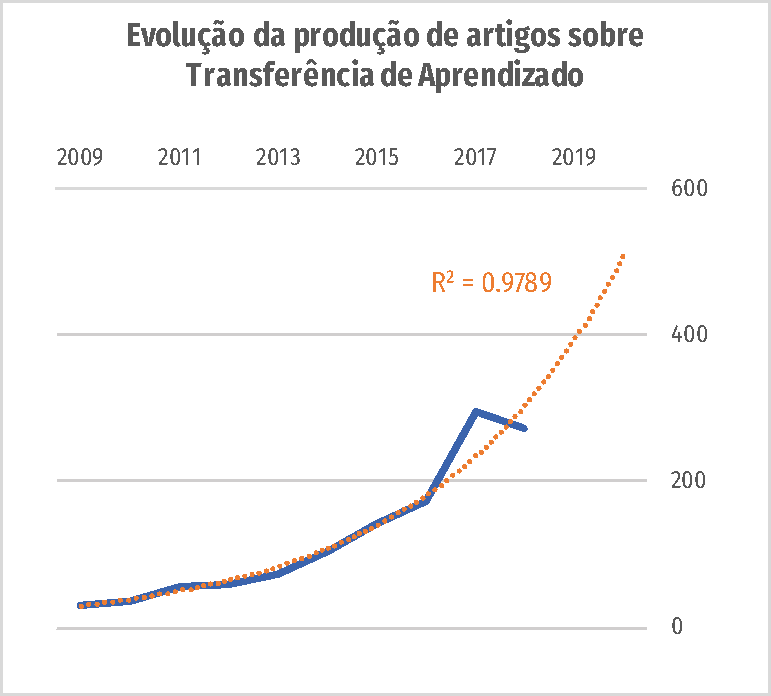
\includegraphics[width=\columnwidth]{artigos_por_ano}
    \source{Web of Science (março/2019)}{Excel}
    \caption{Evolução do número de artigos em Tranferência de Aprendizado nos últimos 10 anos. Até 2021, o número de artigos na área deverá dobrar.}
    \label{fig:artigos_por_ano}
  \end{figure}

  Em 2012, a rede neural profunda\footnote{deep neural network} submetida pelo time de Alex Krizhevsky et. al. para o desafio Imagenet (ILSVRC) performou 41\% melhor que o segundo colocado, dando início ao crescimento explosivo de \emph{deep learning}. Tal sucesso ressaltou a importância dos dados para o avanço de inteligência artificial, mas também permitiu uma igual quebra de paradigma em transferência de aprendizado: percebeu-se que modelos treinados na ImageNet podiam facilmente ser usados para inicializar outros modelos e reduzir em muito a necessidade de amostras~\cite{Ruder2019Neural}.   Essa abordagem de "sintonia fina"\footnote{\emph{fine-tuning}} permitiu resultados bons em diversas tarefas com ordens de magnitude a menos de dados (vide \S\ref{terceira_onda}). 

  Atualmente, \emph{transferência de aprendizado} é um tópico comum em prestigiadas conferências como CVPR, ICCV, ICPR e NeurIPS (vide figura \ref{fig:toptop}, \emph{Top 10 encontros}).
  \subsection{Notações e definições}
  \begin{figure}[h]
    \fbox{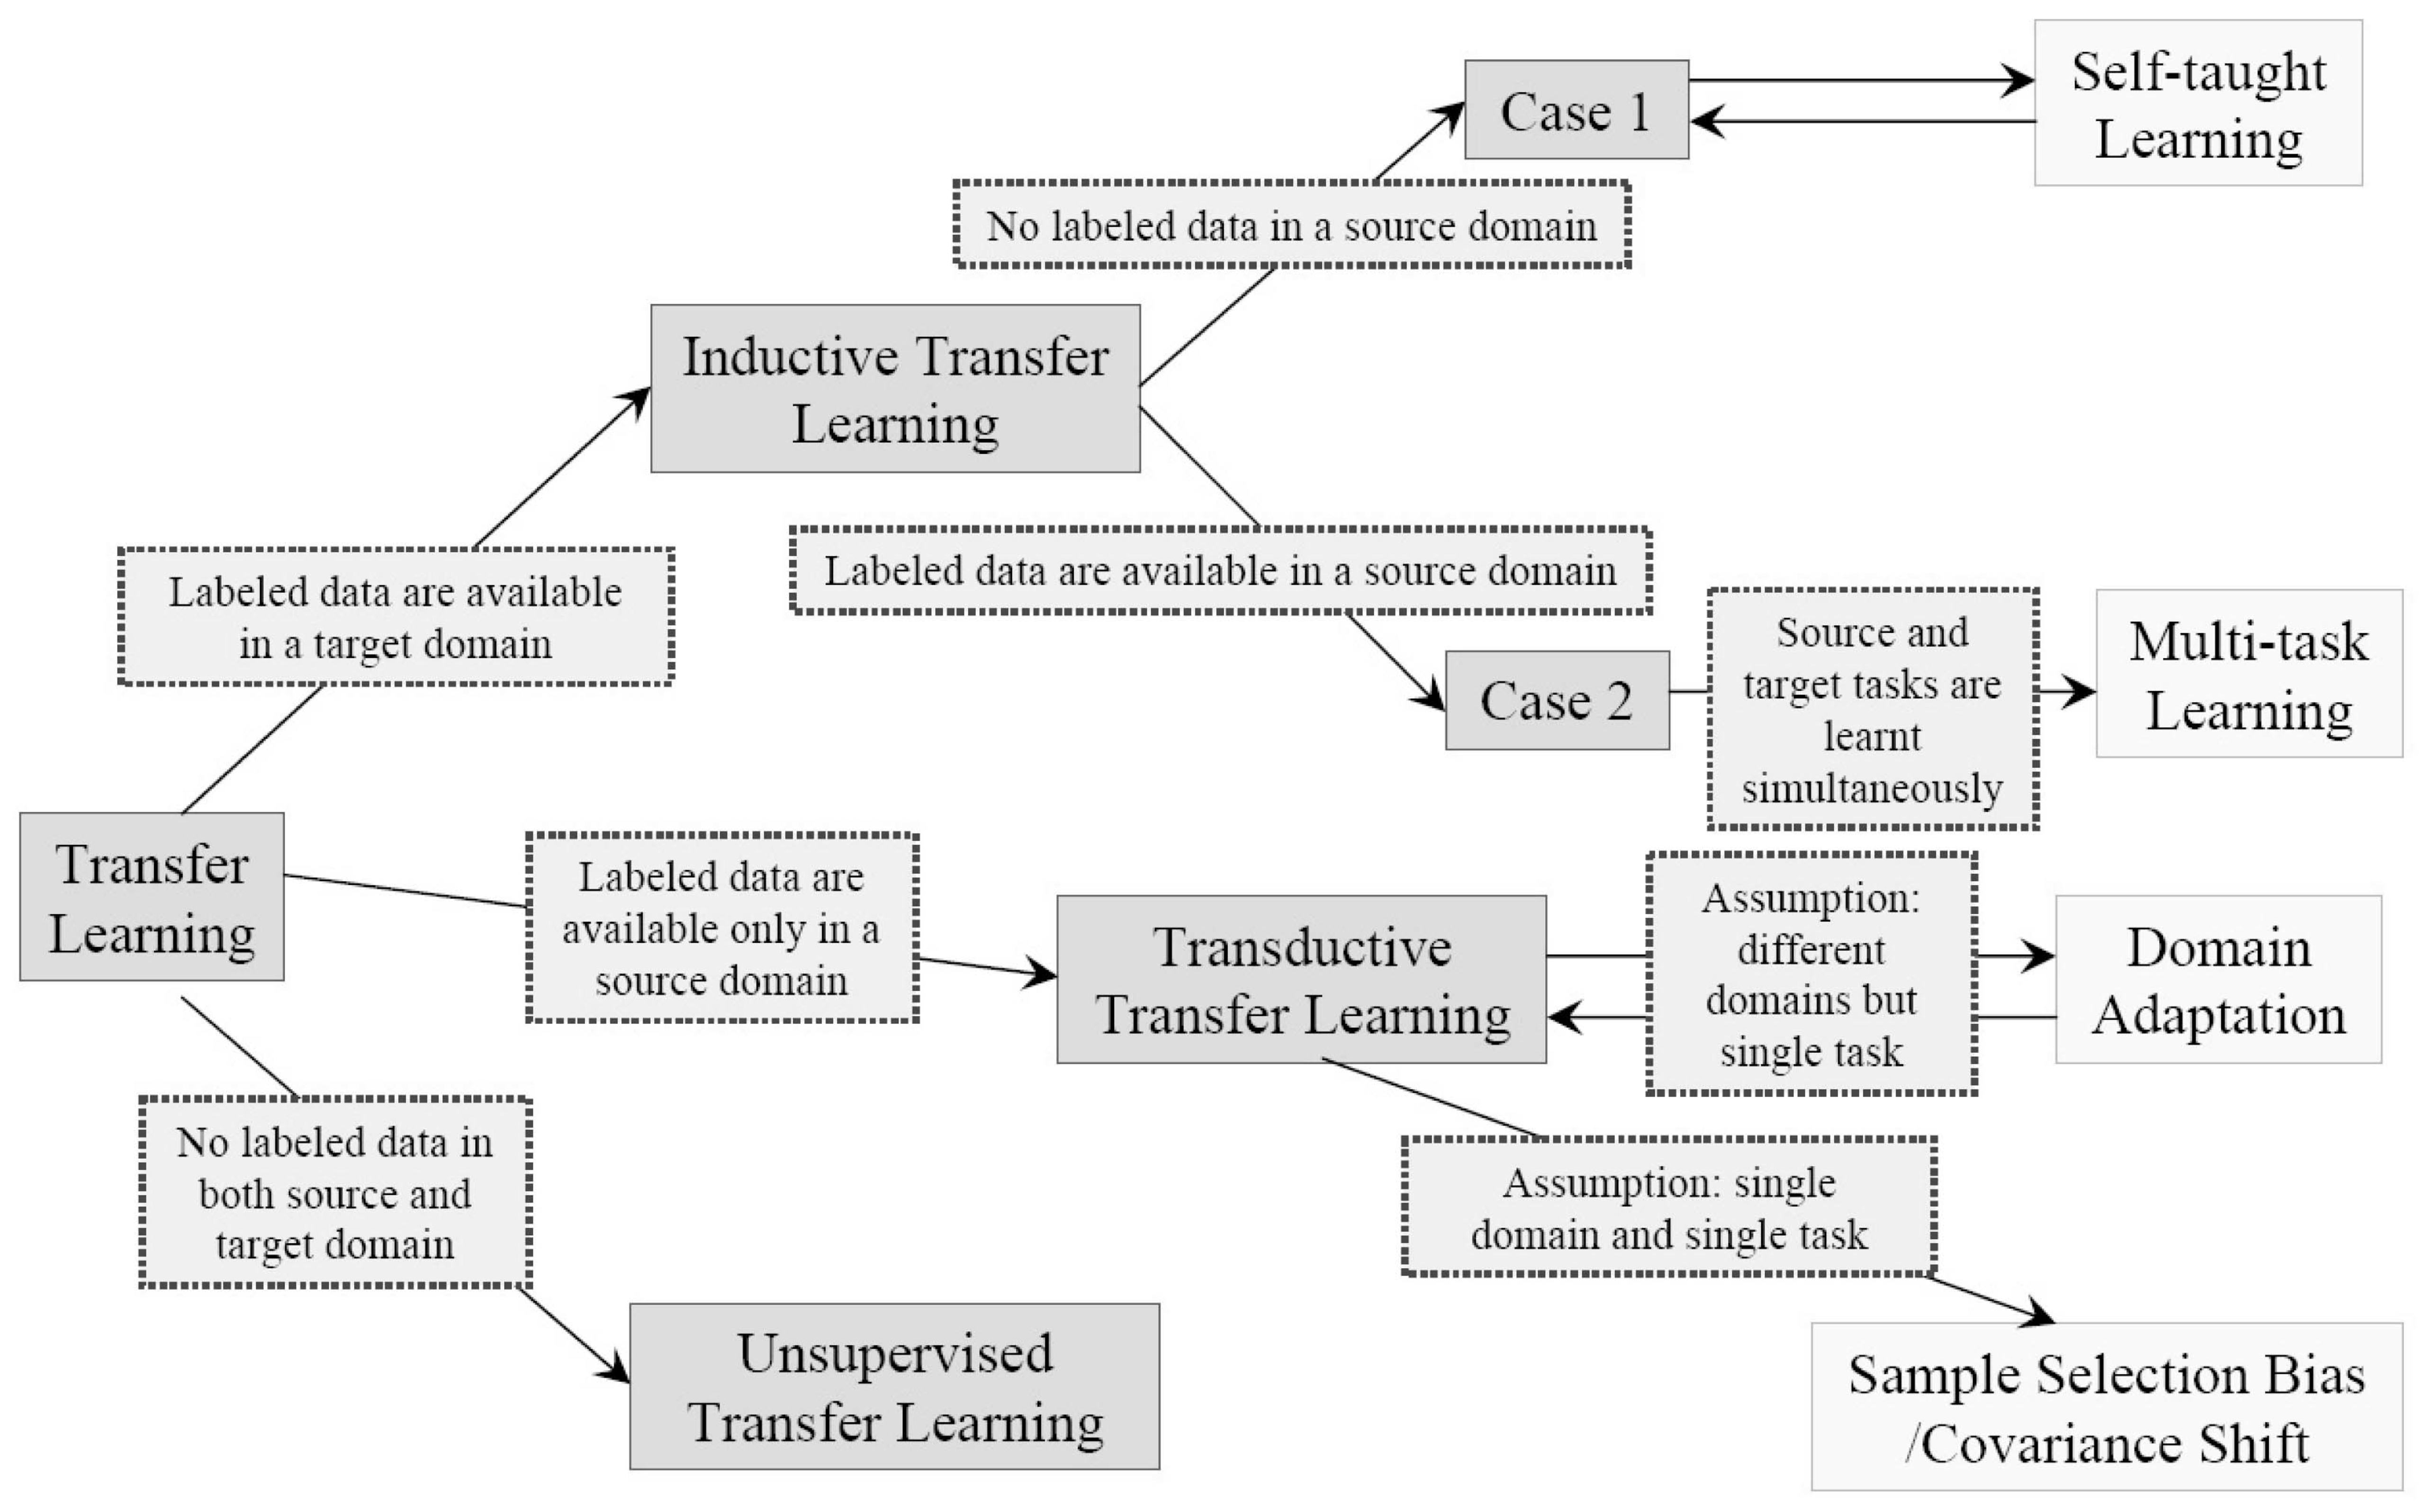
\includegraphics[width=\columnwidth]{taxonomy.pdf}}
    \caption{Visão geral dos diversos tipos de transferência. Taxonomia de \emph{A Survey on Transfer Learning}\protect{~\cite{PanYang}} }
    \label{fig:taxonomia}
  \end{figure}
    Transferência de aprendizado envolve os conceitos de \emph{domínio} e \emph{tarefa}. Seguindo a notação de \cite{PanYang}, um domínio $\mathcal{D}$ é composto de um espaço de características $\mathcal{X}\subset R^d$ e uma distribuição marginal $P(\mathrm{X})$, onde $\mathrm{S}=\{x_1, \dots, x_n\}\in\mathcal{X} $. Para um problema de classificação de imagens, por exemplo, $\mathcal{X}$ é o espaço de todas possíveis representações de imagens, com suas dimensões e canais, $x_i$ é uma imagem e $\mathrm{S}$ é o \textit{dataset} de treinamento. 

    Dado um domínio $\mathcal{D}=\{\mathcal{X}, P(X)\}$, uma tarefa $\mathcal{T}$ é definida pelo espaço de rótulos $\mathcal{Y}$ com distribuição condicional $P(\mathrm{Y}|\mathrm{X})$, ou seja, $\mathcal{T}=\{\mathcal{Y}, f(\cdot)\}$, onde $f(\cdot)$ é uma função objetivo que dado um $x_i \in \mathcal{D}$, prediz seu correspondente $y_i \in \mathcal{Y}$. 

    Dado um domínio fonte $\mathcal{D_S}$ e uma tarefa $\mathcal{T_S}$, um domínio destino $\mathcal{D_T}$ e uma tarefa $\mathcal{T_T}$, \textbf{transferência de aprendizado} objetiva auxiliar o aprendizado da função de predição $f_T(\cdot)$ em  $\mathcal{D_T}$ usando conhecimento de $\mathcal{D_S}$ e $\mathcal{T_S}$, onde $\mathcal{D_S}\neq\mathcal{D_T}$ ou $\mathcal{T_S}\neq\mathcal{T_T}$.

    No presente artigo, usaremos a taxonomia apresentada por \cite{PanYang} (figura \ref{fig:taxonomia}). 
    \subsection{O panorama da produção científica na área}\label{sec:panorama}
  Na figura \ref{fig:toptop}, Top 10 autores, é possível notar que o autor com mais citações é Pan, S., com 2706 citações. Tal impacto deve-se, sobretudo ao artigo \emph{A Survey on Transfer Learning}, que é o artigo mais citado da área com 2240 citações. O mérito deste trabalho é apresentar definições, notações e uma taxonomia para TL. Saiu na revista \emph{IEEE Transactions on Knowledge an Data Engineering}, de 2,775 de fator de impacto, e ocupa a 33\textordfeminine ~posição no ranking de publicações InCite JCR para a categoria \emph{Computer Science, Artificial Intelligence}, ou seja, uma publicação cujo foco não é o tipo de pesquisa que menciona \emph{transferência de aprendizado}. 

  A China é o país com o maior número de artigos publicados, seguido pelos Estados Unidos. O Brasil está na 11\textordfeminine ~colocação, junto com a Índia, mas a frente de países como Espanha, Coreia do Sul e Israel.

  A maior parte dos artigos são publicados em \emph{proceeding} de conferências, 63\%. A conferência com mais artigos sobre TL é a CVPR\footnote{Conference on Computer Vision and Pattern Recognition}, mas a ECCV\footnote{European Conference on Computer Vision}, apesar de ser somente a 4\textordfeminine em artigos,  é a conferência com o maior número agregado de citações. É digno de nota que as conferências de visão computacional tem sido o espaço onde artigos de TL mais são divulgados. Ao mesmo tempo, estranha a falta de alguma conferência com maior foco em NLP. Também não há entre os 20 artigos mais citados, nenhum que seja especializado em linguagem.
  \subsection{Os Clássicos}\label{classicos}
  \begin{figure}[h!]
    \fbox{\includegraphics[width=\columnwidth]{completo_21.pdf}}
    \source{Web of Science (março/2019)}{VosViewer\protect{~\cite{VOSviewer}}}
    \caption{Núcleos de conhecimento obtidos pela análise de co-citações. Os diferentes grupos representam autores que normalmente são co-citados nos 1268 artigos resultantes da busca realizada.}
    \label{fig:classicos}
  \end{figure}
  \begin{figure*}[htp]
    \centering
    \fbox{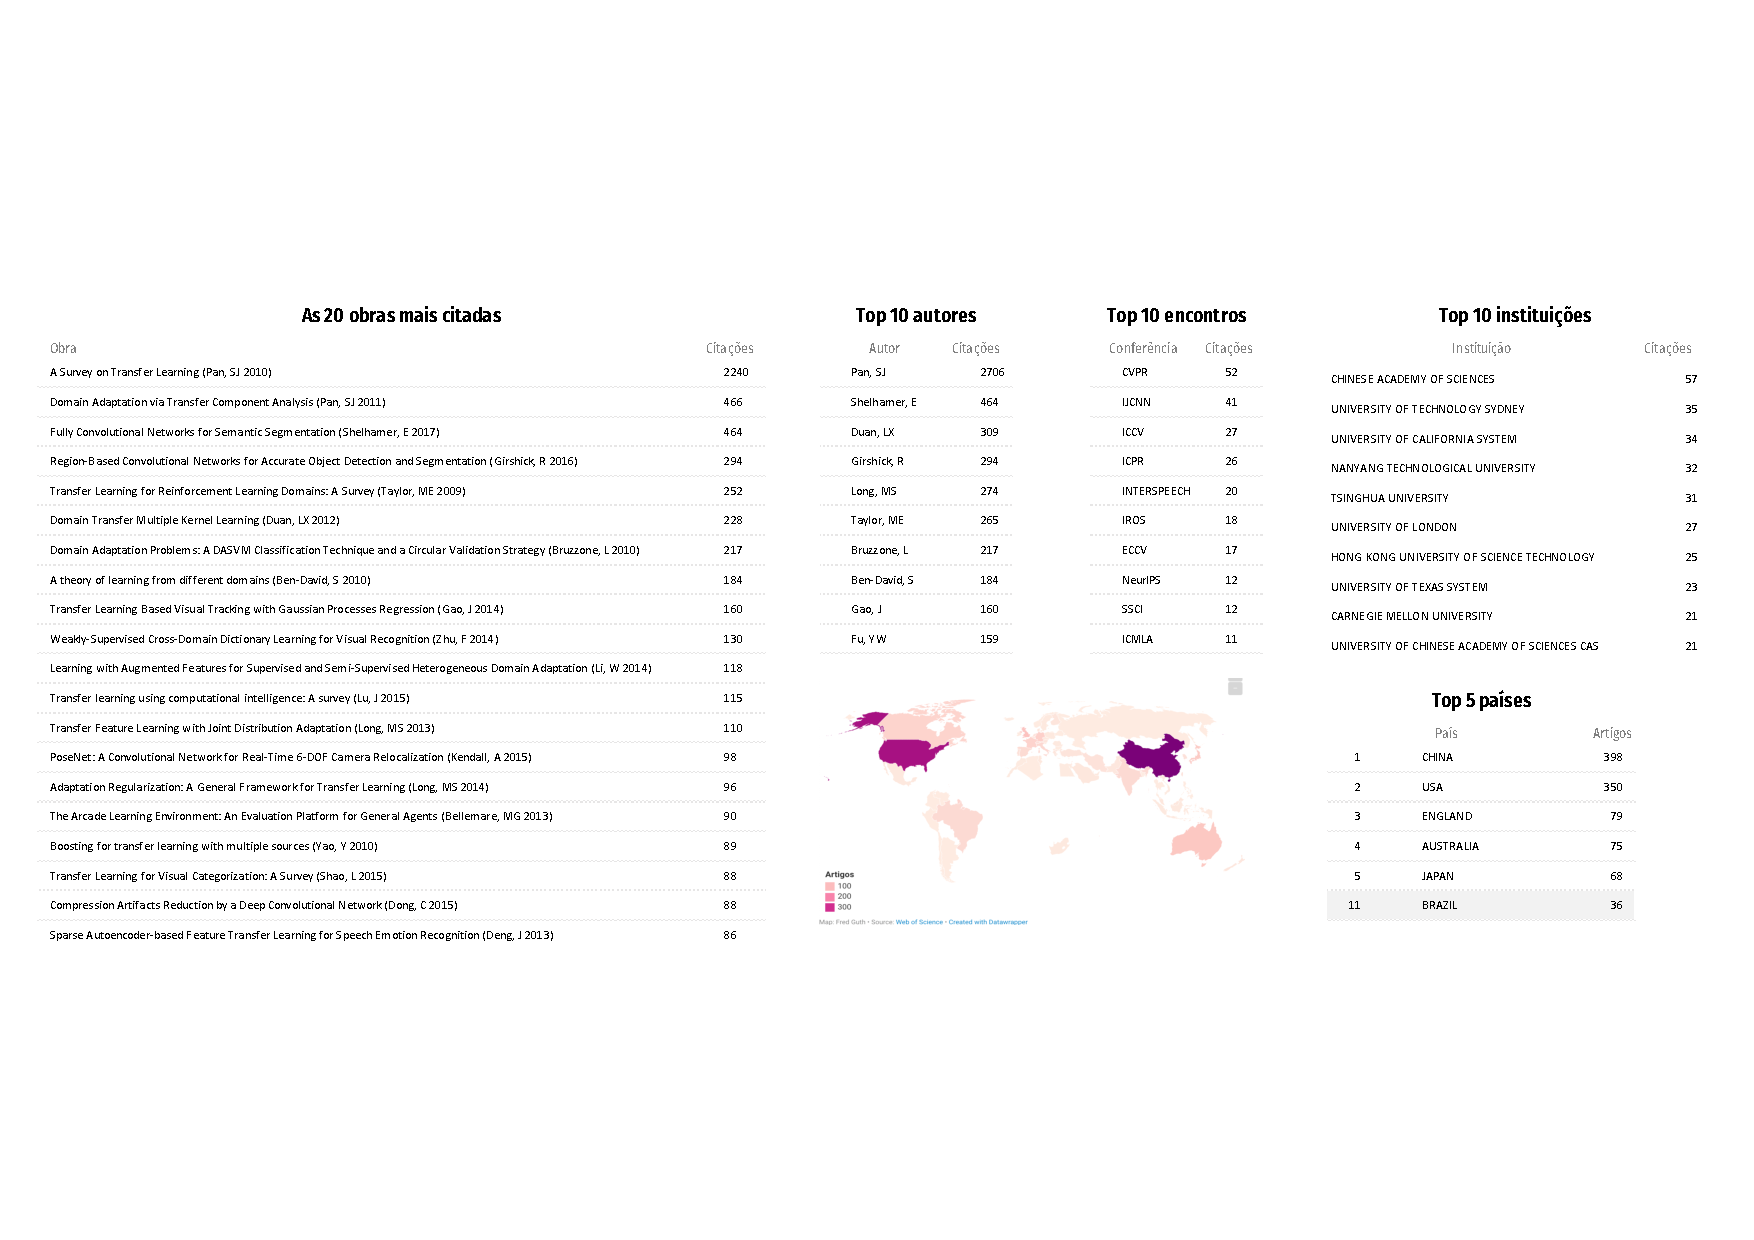
\includegraphics[width=\textwidth]{listas.pdf}}
    \source{Web of Science (março/2019)}{Excel}
    \caption{Panorama da produção científica sobre Transferência de Aprendizado.} \label{fig:toptop}
  \end{figure*}
A análise de co-citação usando o \emph{VosViewer} apontou para existência de 3 núcleos\footnote{\emph{clusters}} de conhecimento. Esses núcleos têm um forte componente temporal, podendo ser vistos como ondas: a primeira concentrando obras anteriores a 2011 (a moda é 2006),  está em amarelo na figura \ref{fig:classicos}; a segunda entre 2011 e 2014 (a moda é 2012) está em vermelho; e a terceira e última onda, em verde na figura, são obras de 2012 até hoje (moda 2014).

\subsubsection{Primeira onda}\label{primeira_onda}
Uma das características mais fortes desta onda é sua componente teórica. Nesse núcleo estão obras que apresentam algumas classes de transferência de aprendizado: Thurn, S. (1996) \cite{thrun1996learning} e Caruana, R. (1997) \cite{Caruana1997} introduzem \emph{Multi-Task Learning} e a ideia de que tarefas auxiliares introduzem um viés indutivo que facilita a convergência do aprendizado; Chapelle, O. (2006) \cite{Chapelle:2010:SL:1841234} com seu livro sobre \emph{Semi-Supervised Learning}; Raina, R. (2007) e \emph{Self-taught learning}; Vapnik, V. (1998) \cite{Vapnik1998} e os fundamentos da teoria de aprendizagem estatística.

Uma outra componente da primeira onda são artigos de Adaptação de Domínio, com certo foco em abordagens que buscam aprender características latentes, de menor dimensionalidade, com o pressuposto que em um espaço latente os domínios são mais similares: Ando, R. K.(2005) \cite{ando2005framework}, Blitzer, J. (2006) \cite{Blitzer:2006:DAS:1610075.1610094} e Daume, H. (2006) \cite{DaumeIII2006}, por exemplo. 

Por fim, algumas das obras mais citadas desta onda são \emph{surveys}: Pan, S. (2010) \cite{PanYang}, Taylor, M. E. (2009) \cite{Taylor:2009:TLR:1577069.1755839}; que não por coincidência aparecem já mais para o final da primeira onda, organizando a pesquisa até aquele ponto. 

\subsubsection{Segunda onda}\label{segunda_onda}
A segunda onda é dominada por artigos sobre Adaptação de Domínio.  Alguns continuam com o foco em características latente como Pan, S. (2011) \cite{Pan2011}, mas a maioria usa abordagens que tentam selecionar amostras do domínio fonte que sejam similares ao domínio alvo: Ben-David, S. (2010) \cite{BenDavid2009} aborda similaridade da distribuição de domínios, Si, S. (2010) \cite{SiSi2010} busca minimizar a divergência; Nesta abordagem também é comum utilizar classificadores, em geral \emph{Support Vector Machines} (SVMs): Yang, J. (2007) \cite{Yang2007}, Bruzzone, L. (2010) \cite{Bruzzone2010}, Duan, L. (2012)\cite{LixinDuan2012}, entre outros.

Há também trabalhos de Adaptação Não Supervisionada de Domínio: Gong, B. (2012) \cite{BoqingGong2012}, Fernando, B. (2013) \cite{Fernando2013}.
Notou-se com estranheza que não apareceu em nossa análise nenhuma \emph{survey} "fechando" essa onda, apesar de sabermos da existência do capítulo \emph{A Comprehensive Survey on Domain Adaptation for Visual Applications}, Csurka, G. (2017) \cite{Csurka2017}. Foi constatado, entretanto, que esta obra não foi indexada pela base \emph{WoS} e portanto não fez parte dos resultados de nossas buscas. 

\subsubsection{Terceira onda}\label{terceira_onda}
A terceira onda é o núcleo de conhecimento de transferência de aprendizado no contexto de \emph{deep learning}, que podemos chamar de \emph{deep transfer learning}. 

Encontramos obras clássicas como: Hinton, G. (2006) \cite{Hinton2006}, talvez o artigo seminal de \emph{Deep Learning}; Bengio, Y. (2009) \cite{Bengio2009} apresenta o conceito de \emph{representation learning} e a ideia de curriculum, uma lista de tarefas a serem aprendidas em sequencia, por terem representações em crescentes níveis de complexidade; LeCun, Bengio e Hinton (2015)\cite{LeCun2015} fazem uma revisão da área de \emph{Deep Learning}. Também aqui se encontra o artigo de Krizhevsky, A. (2012) \cite{alexnet}, sobre \emph{AlexNet}, o modelo que, ao ganhar o desafio ImageNet (ILSVRC) de 2012 com uma margem de mais de 40\% acima do segundo colocado, tornou \emph{Deep Learning} conhecido do público geral e deu início a uma verdadeira "corrida do ouro" ~na pesquisa de aprendizado de máquina. 

Alguns artigos são sobre \emph{large datasets}, um importante componente de \emph{deep learning}:  Deng, J. (2009) \cite{Deng2009} apresenta a ImageNet e sugere que modelos treinados nela poderão ser usados para aprender novos domínios mais facilmente; Everingham, M. (2009) \cite{Everingham2009} traz o desafio Pascal VOC; Russakovsky, O. (2015) \cite{Russakovsky2015} analisa o impacto da ImageNet em diversos problemas de visão computacional, e, consequentemente, o papel da transferência de aprendizado. 

Há também artigos que apresentam arquiteturas para resolução de tarefas específicas, utilizando modelos pre-treinados na ImageNet como extração de características: Girshick, R. (2014) \cite{Girshick2014}, modelo R-CNN, He, K. (2016) \cite{He2016}, Resnet, e Simonyan, K.\cite{simonyan2014very}, em detecção de objetos;  Fan, J. \cite{JialueFan2010} em rastreamento de humanos; Long e Shelhamer (2015) \cite{Long2015} em segmentação semântica; entre outros.

Transferência de aprendizado passou a ser tão onipresente em \emph{Deep Learning} que Mahajan, D. (2018) \cite{mahajan2018exploring} argumenta que \emph{não} pré-treinar modelos na ImageNet em problemas de visão computacional é um descuido.  

Por essa razão, é difícil apontar trabalhos desta onda cujo foco seja apenas transferência de aprendizado. Nessa vertente, alguns artigos dignos de nota são: Glorot, X. (2011) \cite{glorot2011domain} é o primeiro a propor aplicar \emph{deep neural networks} par aprender representações comuns entre domínios; Donahue, J. (2014)\cite{donahue2014decaf} e Oquab, M. (2014)\cite{Oquab:2014:LTM:2679600.2680210} mostram que parâmetros aprendidos em tarefas fonte servem como representações que permitem aprender com poucos exemplos a tarefa alvo, dando um embasamento teórico a técnica mais largamente utilizada na prática, sintonia fina. 
\subsubsection{Resultados da análise textual}
Os 20 artigos mais citados representam quase metade das citações (figura \ref{fig:citacoes_por_ano}). Assim, assumimos que uma análise textual nesse subconjunto da "Busca10Anos" é um bom \emph{proxy} do conjunto dos artigos. 

A figura \ref{fig:scatterText_documentbased} apresenta os 20 artigos mais citados visualizados por proximidade dos termos contidos nos \emph{abstracts} e \emph{keywords} dos mesmos.  Os eixos são os dois termos com maior \textbf{tf-idf}. Quando o artigo faz parte de algum dos núcleos clássicos (figura \ref{fig:classicos}), representamos o seu ponto no gráfico com a mesma cor do núcleo clássico do qual faz parte.
É interessante notar, que em linhas gerais, por um método totalmente diferente, agrupamos nos mesmos núcleos os artigos. Na figura \ref{fig:scatterText_documentbased}, cada quadrante equivale a um núcleo da figura \ref{fig:classicos}.  Essa é uma forte validação das análises.

A figura \ref{fig:clouds} apresenta "nuvens de palavras" para cada quadrante da figura \ref{fig:scatterText_documentbased}. É interessante notar que esses termos validam a análise feita na seção \S\ref{classicos}.

\begin{figure}
  \fbox{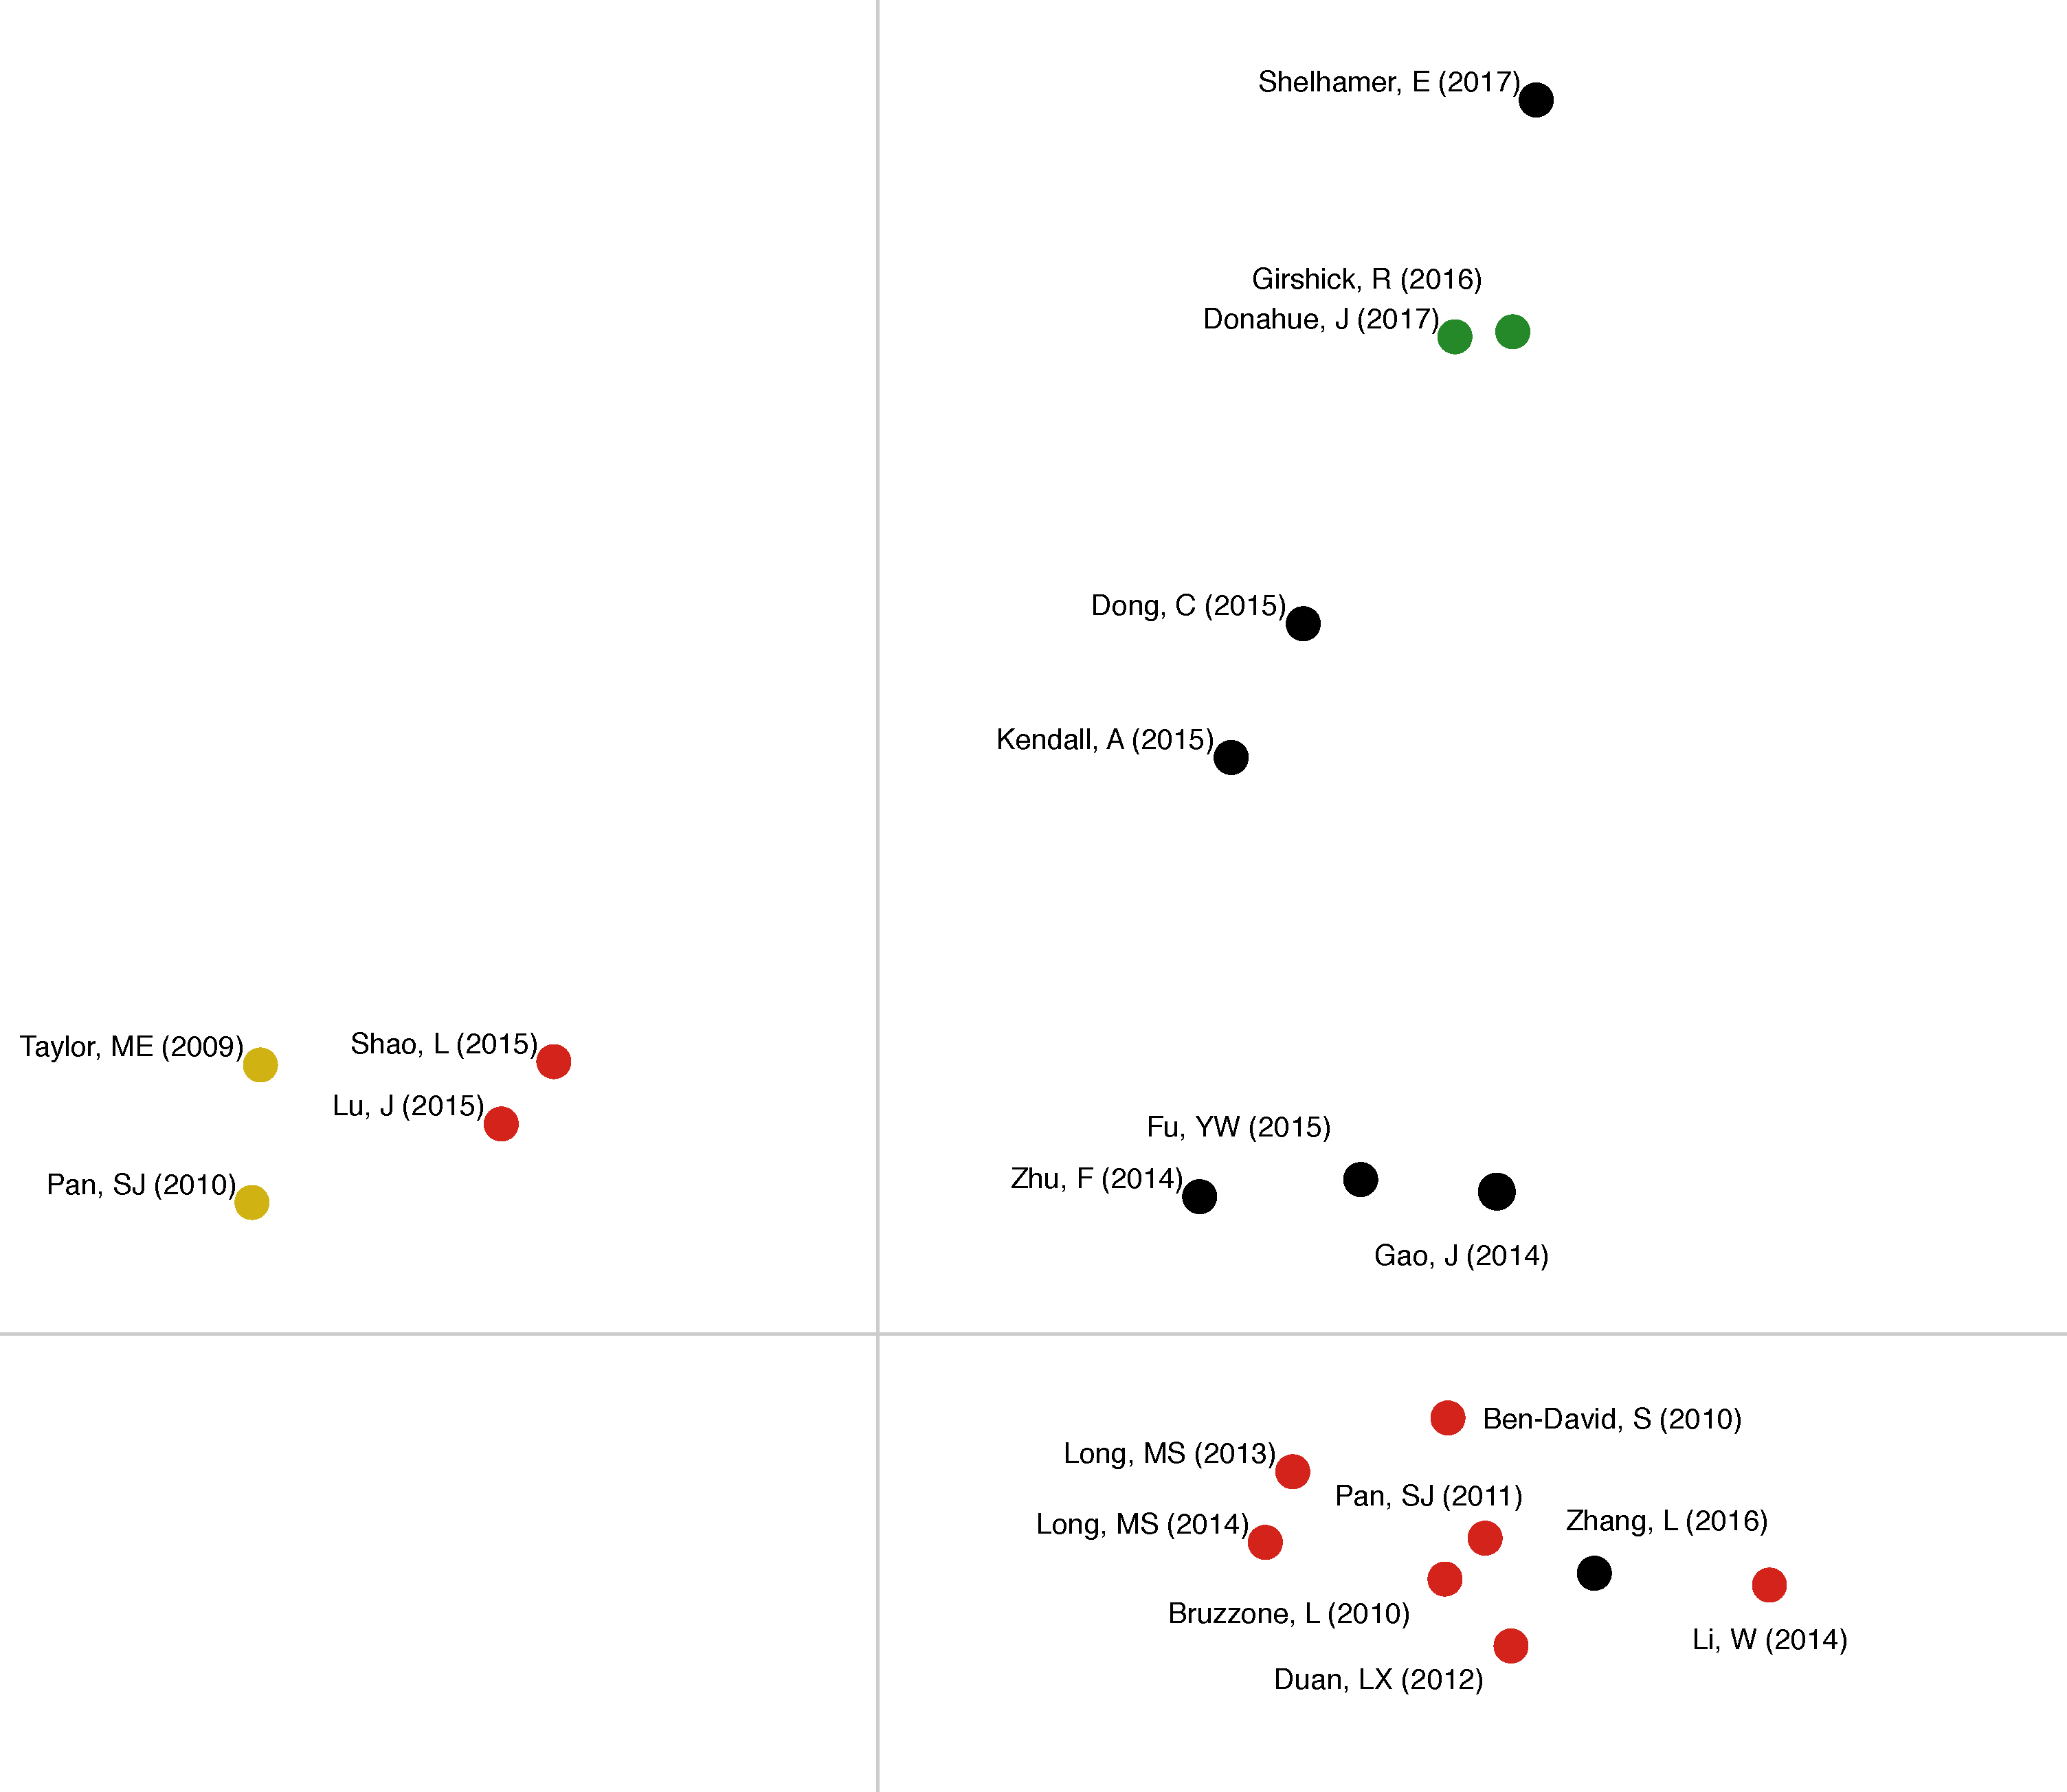
\includegraphics[width=\columnwidth]{top20_abstracts.pdf}}
  \source{WoS (março/2019)}{ScatterText~\protect{\cite{kessler2017scattertext}}}
  \caption{Os 20 artigos mais citados visualizados por proximidade de \emph{bag of words}.} \label{fig:scatterText_documentbased}
\end{figure}
\begin{figure}
  \fbox{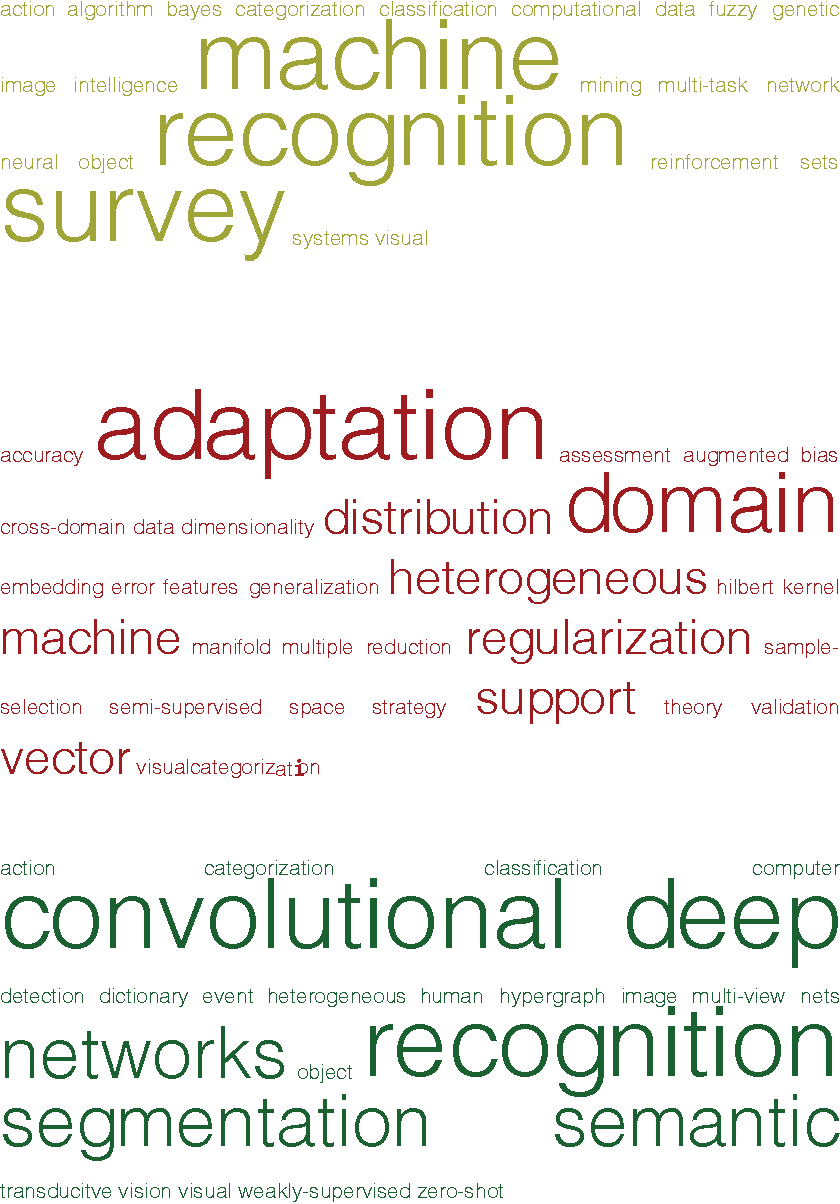
\includegraphics[width=\columnwidth]{keyword_clouds}}
  \source{WoS (março/2019)}{TagCrowd}
  \caption{Nuvens de palavras dos diferentes quadrantes da figura \ref{fig:scatterText_documentbased}.} \label{fig:clouds}
\end{figure}


\subsection{As Fronteiras}\label{fronteiras}
  Pra caracterizar as fronteiras de pesquisa em transferência de aprendizado fizemos duas análises:
  \subsubsection{Análise Textual}

  Utilizamos o \emph{ScatterText}~\cite{kessler2017scattertext} para analisar as diferenças dos termos que representam os artigos da  "Busca3anos", que são mais prováveis de estar na fronteira de pesquisa, com os termos da "Busca10Anos", que engloba todos os artigos sobre TL. 

  O resultado é apresentado na figura \ref{fig:scatterText}. 
  É interessante notar que os termos mais identificados com as fronteiras são \emph{deep}, \emph{neural}, \emph{images} e também palavras como \emph{cnn},  \emph{trained networks} e \emph{datasets}.  O que tem bastante correspondência com a noss análise da terceira onda em \S\ref{terceira_onda}. Já os termos da "Busca10Anos" são: \emph{distribution}, \emph{domain}, \emph{adaptation}, \emph{auxiliary} (de tarefas auxiliares), \emph{kernel}; bastante similariedade com a segunda onda \S\ref{segunda_onda}. 

  \begin{figure}
    \includegraphics[width=\columnwidth]{frontier.pdf}
    \source{\emph{WoS}(março/2019)}{ScatterText\protect{\cite{kessler2017scattertext}}}
    \caption{Análise visual dos termos mais "Fronteira" versus os termos mais "Clássico" no âmbito de Transferência de Aprendizado.} \label{fig:scatterText}
  \end{figure}

  \subsubsection{Acoplamento Bibliográfico}
  O resultado do acoplamento bibliográfico dos artigos da "Busca3anos" pode ser analisado na figura \ref{fig:bicoupling}.
  \begin{figure}[b]
    \fbox{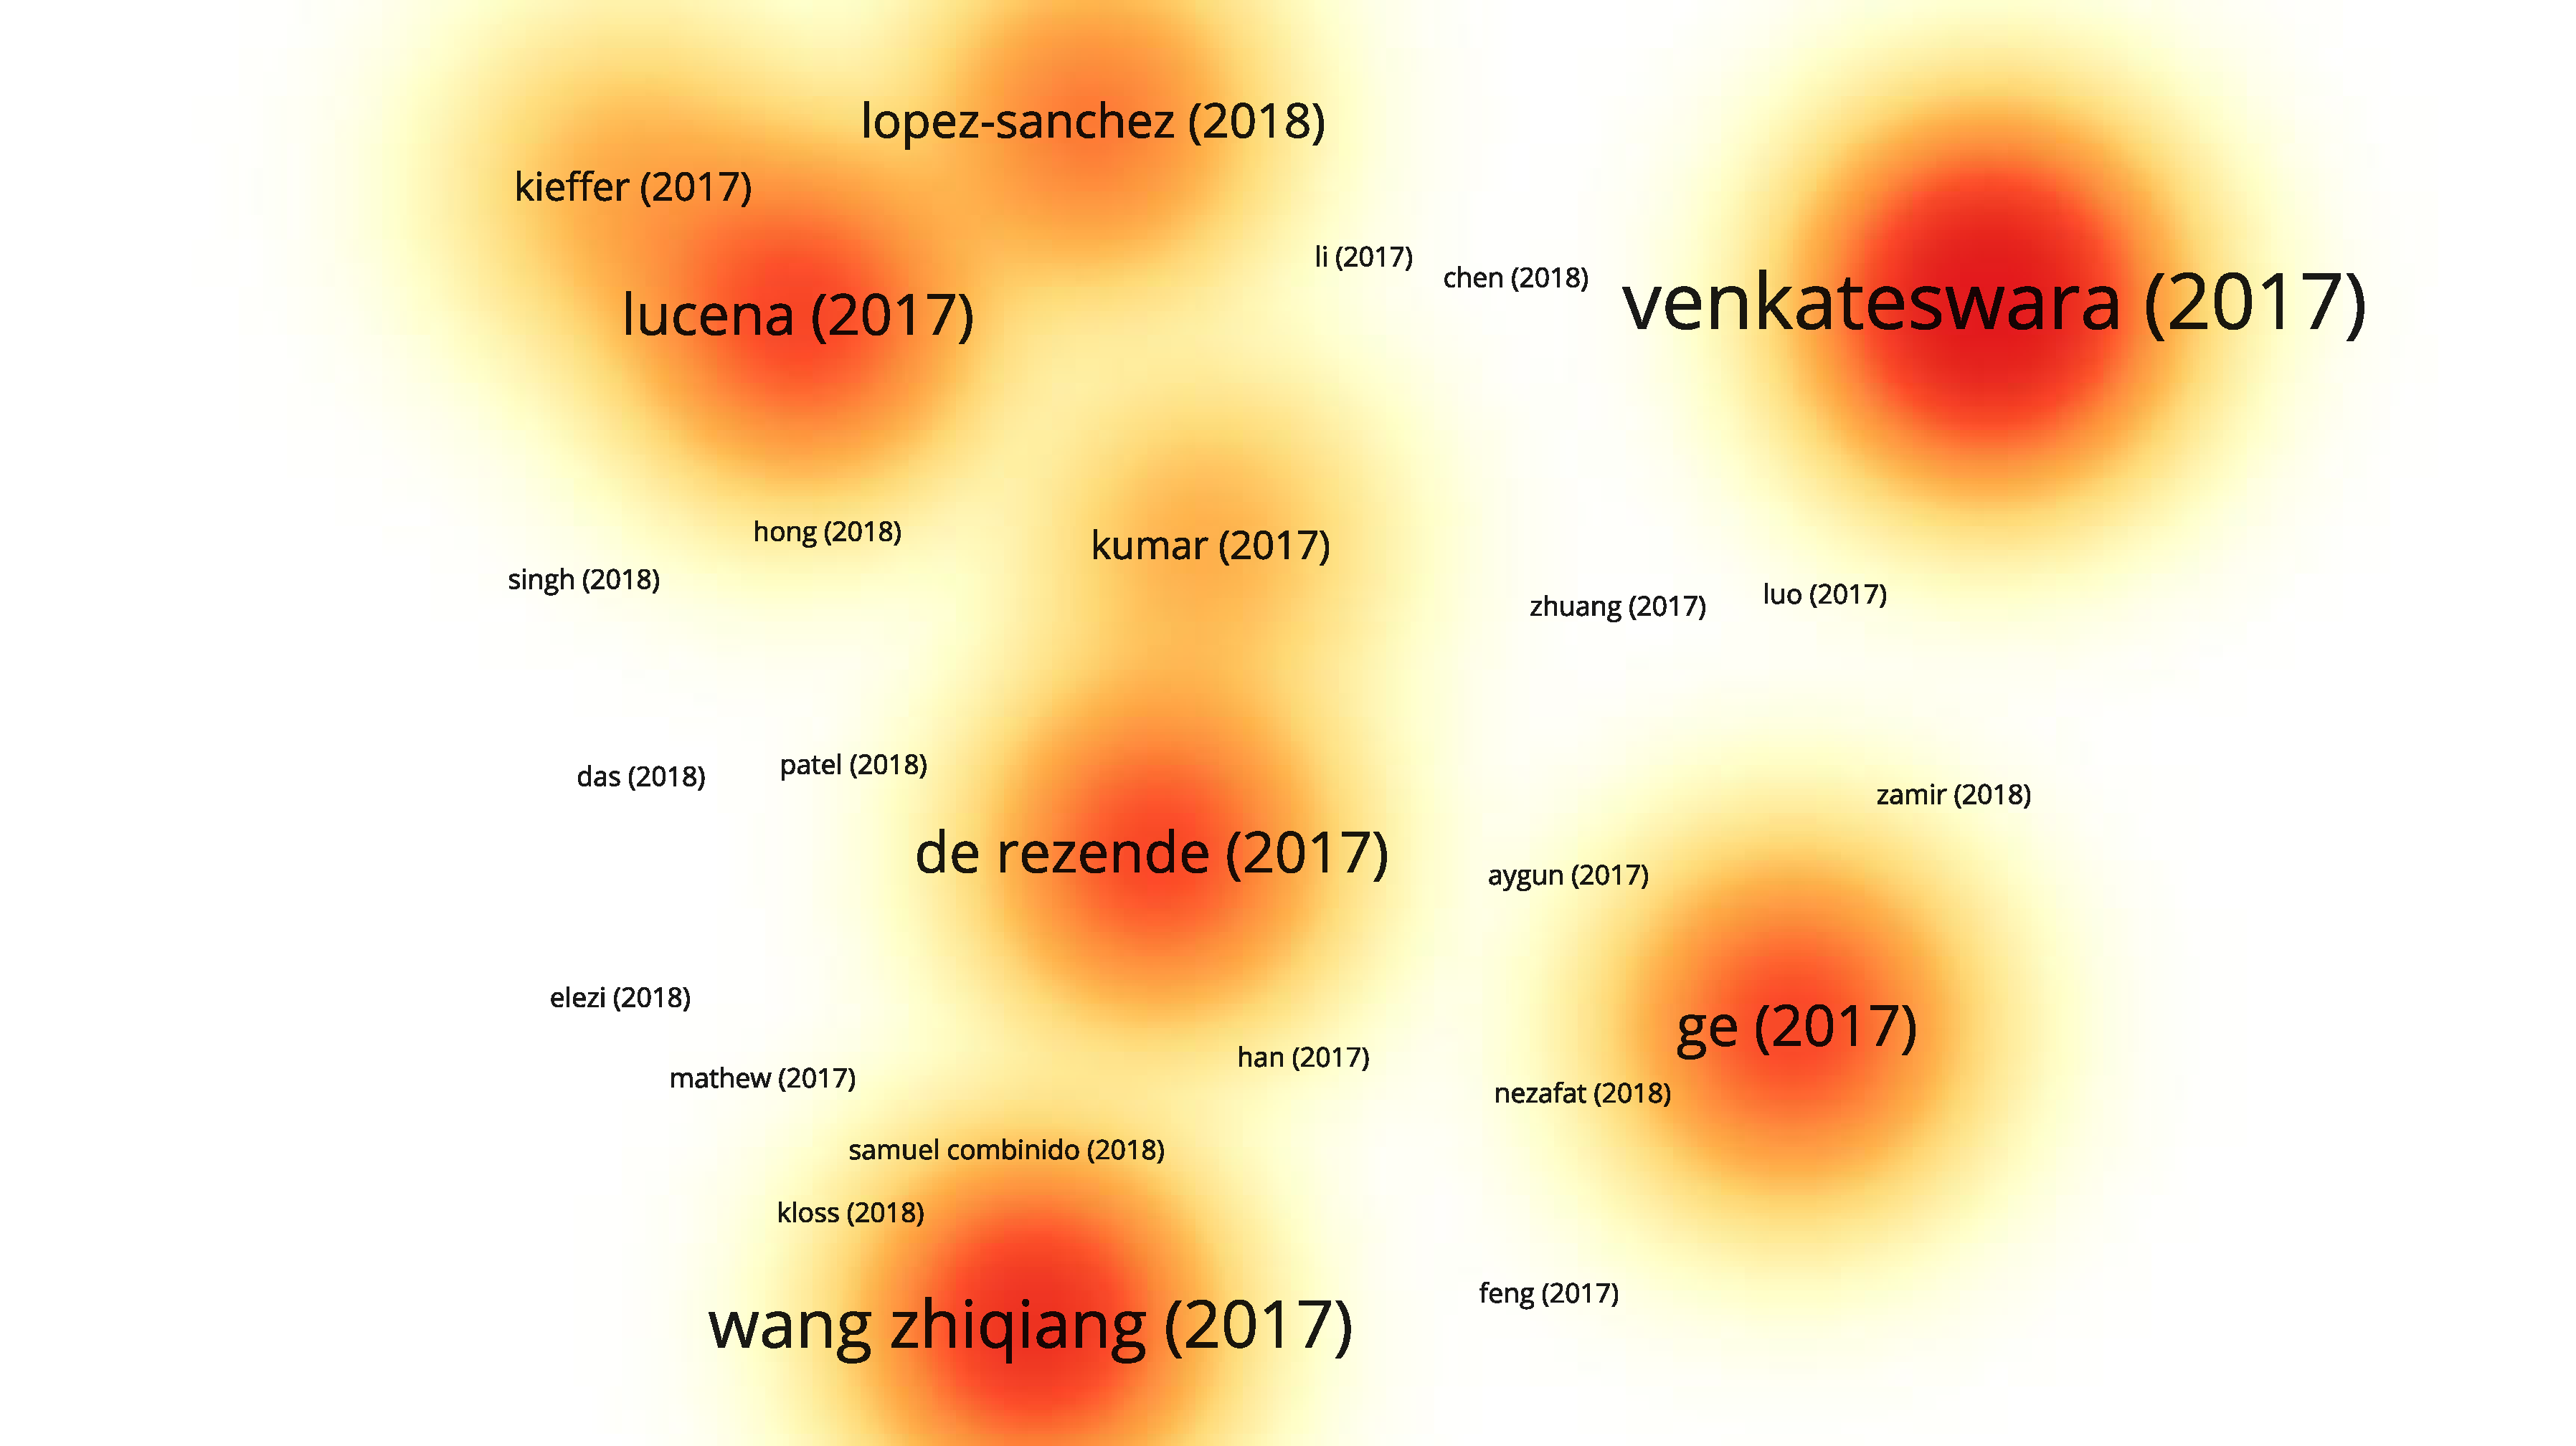
\includegraphics[width=\columnwidth]{frontier_heat}}
    \source{\emph{WoS}(março/2019)}{VosViewer}
    \caption{Mapa de calor da análise de acomplamento bibliográfico.} \label{fig:bicoupling}
  \end{figure}

  Analisando os artigos mais destacados, temos:
  Lucena, O. (2017) \cite{Lucena2017} e de Rezende, E. (2017) \cite{Rezende2017}, ambos artigos brasileiros, são aplicações de \emph{deep convolutional networks} para novos problemas, \emph{face anti-spoofing} e \emph{identificação de fake images}, respectivamente.
  Venkateswara, H. (2017) \cite{Venkateswara2017} e Ge, W. (2017)\cite{Ge2017} propõem novos métodos de Adaptação de Domínio usando \emph{Deep Learning}. 
  Fica claro que o aspecto em comum de todos esses trabalhos é que são exemplos de \emph{Deep Transfer Learning}.

  \subsubsection{Os clássicos de amanhã}
  As análises quantitativas, apontam grande potencial em \emph{Deep Transfer Learning}, mas não são capazes de sugerir se esse ou aquele trabalho é ou não promissor.  Para tanto, além de escolher trabalhos com as características mais "quentes", também é necessária uma análise subjetiva dos trabalhos que parecem estar avançando em espaços em aberto. 
  
  Nesse espírito, ressaltamos algumas obras que acreditamos ter potencial para se tornarem clássicos de amanhã:
  \begin{itemize}
    \item Zamir, A. (2018)\cite{taskonomy}: considerado o melhor artigo da CVPR 2018, esse artigo explora as relações entre tarefas, criando um grafo que pode ser utilizado para definir que tarefas são as melhores fontes para uma determinada tarefa alvo, entre outras questões.
    \item Howard, H. (2018)\cite{ulmfit}: o modelo ULMFit avançou o estado-da-arte de tarefas de classificação de texto entre 18 e 24\% e pode se tornar o equivalente em NLP ao que Krizhevsky, A. (2012)\cite{alexnet} foi para visão computacional. 
    \item Zhu, J. (2018)\cite{CycleGan}: propõe o uso de \emph{Generative Adversarial Networks (GANs)} para transferir o domínio de uma imagem para outra de forma totalmente não supervisionada.  Somos extremamente otimistas em relação ao potencial de GANs para transferência de aprendizado.
    \item Ruder, S. (2019)\cite{Ruder2019Neural}: apresenta uma taxonomia mais atual para problemas de transferência de aprendizado em NLP.
  \end{itemize}

\section{Problemas em Aberto}\label{emAberto}
A visão geral que uma revisão sistemática traz, nos permite perceber lacunas no conhecimento científico. Alguns problemas em aberto são:
\begin{enumerate}
  \item inexistência de métricas específicas para transferência: \emph{"models do what you inspect, not what you expect".}
  \item a taxonomia corrente, Pan, S. (2009)\cite{PanYang}, dá ênfase demais a adaptação de domínio e de menos a transferência indutiva de aprendizado. Também precisa ser atualizada para incluir ideias mais recentes como GANs e \emph{autoencoders}. 
  \item NLP: ainda há muito pouco em transferência de aprendizado para NLP, exceção feita a Ruder, S. (2019)\cite{Ruder2019Neural}.
  \item Teoria: na primeira onda, o papel da teoria era apontar caminhos que poderiam dar certo. Hoje há vários caminhos que estão dando certo na prática, mas muito pouco se sabe  o porquê de darem certo. É importante saber esse porquê. 
\end{enumerate}

\section{Conclusão}\label{conclusao}
Nesta revisão sistemática da literatura, vimos que as fronteiras da transferência de aprendizado estão na tendência de \emph{deep transfer learning}, um campo com muitos espaços em aberto e que engloba o uso de \emph{deep learning} para: a) resolução de novos problemas usando tarefas fonte como extração de características para solução de tarefas alvo; b) encontrar representações latentes entre domínios; c) transferir características entre domínios de forma não supervisionada; entre outros. 
Nesse percurso, nos guiamos pelo método de enfoque meta-analítico, utilizando diferentes ferramentas de análise quantitativa para validar nossas conclusões; demonstrando que é possível embasar a avaliação das fronteiras de pesquisa com dados bibliométricos.

No futuro, questões importantes precisam ser adereçadas: Primeiro, a taxonomia base de Pan, S. (2009)\cite{PanYang} já não condiz com a atualidade, dá importância demais ao que era importante na primeira onda \S\ref{primeira_onda} e já não classifica bem os problemas da terceira onda \S\ref{terceira_onda}.  Além disso, o método de revisão merece diversas melhorias: 1) poderia incluir outras bases como a \emph{Scopus} e \emph{Google Scholar}; 2) Podemos ainda alargar os parâmetros de pesquisa incluindo tipos de transferência como: \emph{multi-task learning}, \emph{domain adaptation} e outros nomes que caíram em desuso como \emph{learning to learn} e \emph{lifelong learning}; 3) poderia englobar a sumarização dos principais trabalhos, de preferência adotando um \emph{framework} como o dos cinco W's e um H\cite{hohman2018visual}.
Por fim, faz-se necessário consolidar o arcabouço teórico e "abrir a caixa-preta" da transferência de aprendizado em \emph{deep learning} e avançar ainda mais nas diferentes aplicações.
\bibliographystyle{ACM-Reference-Format}
\bibliography{references}
\end{document}
